\documentclass[11pt]{article}
\usepackage{tikz}
\usetikzlibrary{arrows.meta,positioning}
\usepackage{tabularx}
\usepackage{amsmath,amssymb,bm,graphicx,booktabs,hyperref,geometry}
\geometry{margin=1in}
\hypersetup{colorlinks=true, linkcolor=blue, citecolor=blue, urlcolor=blue}




\title{\textbf{Paper D-11: Supply Chains:\\ A Constraint-Driven Flux Dynamics (CDFD) Perspective}}
\author{Steve Bico Mujjabi, MD\\
\small Independent Researcher\\
\small Founder, Vura Labs\\
\small Kampala, Uganda\\
\small ORCID: 0009-0001-0556-5516}
\date{May 2026}


\newcommand{\EarthSuppPath}{Part\_A\_Earth\_Systems/supplementary/supplementary\_earth\_}
\newcommand{\EngSuppPath}{Part\_B\_Engineered\_Systems/supplementary/supplementary\_eng\_}
\newcommand{\SocSuppPath}{Part\_C\_Socioeconomic\_Systems/supplementary/supplementary\_soc\_}
\newcommand{\DomainSuppPath}{Part\_D\_Domain\_Applications/supplementary/supplementary\_dom\_}
\begin{document}

\maketitle
\newpage


\begin{abstract}
In this paper we apply Adaptive Flux Limitation (AFL) to supply chain dynamics, modelling
goods throughput as constrained transport governed by the potential $\Phi = \Phi_{demand} +
\Phi_{production} + \Phi_{logistics}$ and constraint $C = C_{inventory} + C_{transport} +
C_{supplier}$. The 2021--2022 global supply chain crisis --- generating \$1 trillion in logistics
cost overruns --- is the AFL demonstration event for JIT fragility at planetary scale. The AFL
framework derives optimal inventory safety stock, bullwhip dampening strategies, and resilient
network topology from first principles.

\textbf{Status: Inferred from AFL first principles; quantitative predictions are hypothesis-level.}\\
\textbf{Series tag: Dom-D10}
\end{abstract}

\section*{Symbol Conventions}

\noindent\textbf{CDFD/AFL Part IV symbol convention.}
\begin{center}
{\small
\begin{tabular}{p{0.15\linewidth}p{0.34\linewidth}p{0.41\linewidth}}
\hline
Symbol & Part IV meaning & Cross-domain reading \\
\hline
$\Phi$ & Driving flux or throughput & Energy, matter, signal, capital, information, traffic, force, or biological load entering a system \\
$C$ & Active constraint or capacity burden & Bottleneck, resistance, boundary, scarcity, toxicity, regulation, topology, latency, or load-bearing limit \\
$S$ & Responsiveness or adaptive surface & The system's ability to reconfigure, buffer, route, repair, learn, or preserve function under changing load \\
$M_s$ & Structural memory & Stored damage, hysteresis, inherited topology, institutional memory, trained weights, ecological legacy, or retained state \\
$\Psi_s$ & Adaptive operating ratio $(\Phi/C)\cdot S\cdot M_s$ & Local bookkeeping gauge for constrained operation, overload, recovery, or regime change; not a universal constant \\
$\Lambda$ & Life Number or capstone surplus ratio where explicitly defined & Reserved for Part II-derived life-number notation or synthesis-level surplus measures, never an undefined decoration \\
\hline
\end{tabular}
}
\end{center}

\noindent\textbf{Greek-symbol convention.}
\begin{center}
{\small
\begin{tabular}{p{0.15\linewidth}p{0.34\linewidth}p{0.41\linewidth}}
\hline
Symbol & Local role & Interpretation rule \\
\hline
$\alpha$ & Accumulation or reinforcement coefficient & Sets how fast a pathway, constraint, habit, cascade, or retained structure grows under load \\
$\beta$ & Relaxation, decay, clearance, or washout coefficient & Sets loss, recovery, damping, forgetting, degradation, or return toward baseline \\
$\gamma$ & Coupling, diffusion, redistribution, or transfer coefficient & Sets spread across nodes, layers, tissues, markets, infrastructures, media, or physical phases \\
$\delta,\epsilon$ & Perturbation, tolerance, small offset, or numerical guard & Used only as local thresholds, stability margins, measurement tolerances, or stress increments \\
$\eta,\lambda,\mu,\nu$ & Efficiency, rate, baseline, intensity, or frequency terms & Meaning is fixed by the equation, subscript, and domain-specific proxy in the paragraph where the term appears \\
$\rho,\sigma,\tau,\phi$ & Density/correlation, variability/noise, time-scale, phase, or field terms & Local coefficients only; subscripts bind them to the named pathway, domain, or experiment \\
$\Omega,\Lambda$ & Domain/state space; Life Number where defined & $\Omega$ names a modeled state space; $\Lambda$ carries life-number or synthesis notation only when the paper defines it \\
\hline
\end{tabular}
}
\end{center}


\section{Series Context}

Part I sets the flow--constraint language used here \cite{MujjabiPartI2026}. Part II develops the Life Number and the origins-of-life use of the same notation \cite{MujjabiPartII2026}. Part III applies AFL to biology and medicine \cite{MujjabiPartIII2026}. Part IV \cite{MujjabiPartIV2026}, DOI \url{https://doi.org/10.5281/zenodo.20395901}, is the cross-domain stress test: it asks where the notation clarifies measurement, and where it becomes only a metaphor.

\section{Introduction}


\subsection{The Mujjabi Universal Capacity Law}
Building directly upon the Fundamental Physics (Part I) \cite{MujjabiPartI2026}, the \textbf{Mujjabi Universal Capacity Law} proposes that across all scales---from black hole event horizons to global financial markets and power grids---driving high flux ($\Phi$) against a rigid topological constraint ($C$) can drive system saturation. When $\Phi/C$ approaches critical thresholds, the system does not scale linearly; it undergoes a topological phase transition.

\subsection{The Mujjabi Universal Memory Law}
The \textbf{Mujjabi Universal Memory Law} frames persistent systemic collapse. When a complex network fails to clear its structural memory ($M_s$) and its relaxation parameter decays ($\tau_{relax} \to \infty$), temporary stressors become permanent rigidities. This is the proposed CDFD mechanism behind ecological death, economic depressions, and infrastructural gridlock.


Modern supply chains span 100+ countries and $10^4$+ nodes, delivering $>$80\% of global
consumer goods. The semiconductor supply chain alone involves 50+ countries, 500+ critical
suppliers, and $10^3$+ product variants. Their vulnerability to disruption was demonstrated
catastrophically during 2020--2022: COVID-19 factory shutdowns in Asia triggered container
shipping shortages, port backlogs, semiconductor supply gaps, and consumer good shortages
that persisted for 18--24 months.

AFL provides a unified framework for supply chain dynamics: goods throughput is constrained
transport through a hierarchical network; bottleneck nodes are AFL constraint hubs; disruption
cascade is AFL $\Psi_s^* > 1.2$ propagation; the bullwhip effect is an AFL limit cycle from delayed
constraint updating; JIT systems operate at the AFL $\Psi_s^* = 1.0$ knife-edge with zero resilience.

The AFL supply chain framework connects to all other Part~IV papers: logistics is the physical
infrastructure of trade networks (Paper~27); supply chain disruption is a trigger for systemic
crises (Paper~33); JIT fragility parallels the constraint-removal vulnerability in trophic
networks (Paper~42) and neural systems (Paper~35).

\section{Core Hypothesis}

\begin{center}
\textit{
Supply chains are multi-tier AFL networks in which goods throughput $\Phi$ is constrained by
inventory buffers and transport capacity $C$: $\Psi_s^* \approx 1$ is the efficient delivery regime;
$\Psi_s^* > 1.2$ is the disruption cascade regime; the bullwhip effect is an AFL limit cycle; and
JIT systems are critically fragile because $\Psi_{s,JIT} = 1.0$ leaves zero headroom for
perturbation.
}
\end{center}

AFL supply chain hypothesis: the Ford-Richardson bullwhip model --- where retailers over-order
in response to demand shocks, amplifying signal as it propagates upstream --- is the AFL limit
cycle for a system with time-delayed constraint feedback. The amplification ratio (bullwhip ratio)
is:
\begin{equation}
\text{Bullwhip ratio} = \frac{\text{Var}(J_{upstream})}{\text{Var}(J_{downstream})} = 1 + \frac{2L}{\beta_{reorder}} + \frac{2L^2}{\beta_{reorder}^2},
\end{equation}
where $L$ is the order-to-delivery lead time and $\beta_{reorder}$ is the demand forecast update
rate. AFL derives this from the delay-differential AFL system.
\textbf{Status: Bullwhip derivation is analytic; AFL calibration requires supply chain time-series data.}

\section{Supply Chain Potential Fields}

We define the generalised supply chain potential:
\begin{equation}
\Phi = \Phi_{demand} + \Phi_{production} + \Phi_{logistics}
\end{equation}
where:
\begin{itemize}
    \item $\Phi_{demand}$ --- end-consumer demand potential (retail demand, order backlog, market
          clearing prices; the ultimate driving force for all upstream supply activity; propagates
          upstream through the supply chain with amplification);
    \item $\Phi_{production}$ --- production capacity potential (manufacturing throughput, capacity
          utilisation rate; the primary AFL production flux; constrained by capital equipment,
          labour, and material inputs);
    \item $\Phi_{logistics}$ --- logistics throughput potential (container shipping capacity, trucking
          availability, air freight; the transport AFL flux connecting production to demand; severely
          constrained during 2021--2022 by port backlogs and container imbalances).
\end{itemize}

\section{Supply Chain Constraint Axes}

\begin{equation}
C = C_{inventory} + C_{transport} + C_{supplier} + C_{labour}
\end{equation}

\begin{table}[h]
\centering
\caption{Supply chain constraint axes and AFL roles.}
\begin{tabularx}{\textwidth}{@{}lXX@{}}
\toprule
Constraint axis & Physical substrate & AFL role \\
\midrule
$C_{inventory}$ & Safety stock, warehouse capacity & Buffer against demand/supply mismatch \\
$C_{transport}$ & Shipping, rail, truck capacity & Goods flow rate constraint \\
$C_{supplier}$ & Supplier reliability and redundancy & Input availability constraint \\
$C_{labour}$ & Workforce availability, skill match & Production execution constraint \\
$C_{regulatory}$ & Customs, tariffs, trade law & Compliance-induced throughput friction \\
\bottomrule
\end{tabularx}
\end{table}

\subsection{Adaptive Surface Dynamics: Memory and Responsiveness}

The operating ratio $\Psi_s^*$ is mediated by adaptive surface components:
\begin{equation}
\Psi_s^* = (\Phi/C) \cdot S \cdot M_s
\end{equation}
where $S$ (Surface Responsiveness) and $M_s$ (Surface Memory) evolve as:
\begin{align}
\frac{dS}{dt} &= \kappa_s (\Psi_s^* - S) \\
\frac{dM_s}{dt} &= \Phi S - d_m M_s
\end{align}
These components represent the homeostatic capacity of the system to regulate its own operating ratio through memory and responsiveness.

\section{Flux Law}

Supply chain goods throughput:
\begin{equation}
J_{goods} = -\frac{1}{C}\nabla \Phi
\end{equation}
where $\nabla\Phi$ represents the gradient in demand potential from retail (high $\Phi_{demand}$)
to raw material suppliers (low $\Phi_{demand}$), and $C$ is the composite supply chain constraint.

Hub constraint with spatial diffusion:
\begin{equation}
\frac{dC_{hub}}{dt} = \alpha_{congestion}|J_{inbound}| - \beta_{processing} C_{hub} + \gamma_{network}\nabla^2 C_{hub},
\end{equation}
where the spatial diffusion term $\gamma_{network}\nabla^2 C_{hub}$ represents constraint
redistribution across the supply network --- rerouting from congested hubs to alternative nodes.

\section{Conservation Dynamics}

Supply chain inventory evolves as:
\begin{equation}
\frac{\partial \Phi}{\partial t} = \nabla \cdot \left(\frac{1}{C}\nabla \Phi\right) + S
\end{equation}
where $S$ represents:
\begin{itemize}
    \item \textbf{Production injection}: $S_{production}$ adds goods to the supply pipeline at
          manufacturing nodes;
    \item \textbf{Demand withdrawal}: $S_{retail} < 0$ removes goods at retail nodes;
    \item \textbf{Disruption}: $S_{disruption} < 0$ sudden removal of goods (factory closure,
          port blockage, natural disaster).
\end{itemize}

\section{Adaptive Constraint Dynamics}

Supply chain constraint evolves dynamically:
\begin{equation}
\frac{dC}{dt} = \alpha_{utilisation}|J_{goods}| - \beta_{replenishment} C
\end{equation}
where:
\begin{itemize}
    \item $\alpha_{utilisation}$: constraint stress from throughput (high goods flow depletes
          inventory buffers, saturates transport capacity, and increases supplier lead times);
    \item $\beta_{replenishment}$: constraint replenishment rate (inventory restocking, capacity
          expansion, new supplier qualification; typically $1/\beta_{replenishment} = $ 3--6 month
          lead time for major capacity additions).
\end{itemize}

\subsection{Adaptive Surface Dynamics: Memory and Responsiveness}

The operating ratio $\Psi_s^*$ is mediated by adaptive surface components:
\begin{equation}
\Psi_s^* = (\Phi/C) \cdot S \cdot M_s
\end{equation}
where $S$ (Surface Responsiveness) and $M_s$ (Surface Memory) evolve as:
\begin{align}
\frac{dS}{dt} &= \kappa_s (\Psi_s^* - S) \\
\frac{dM_s}{dt} &= \Phi S - d_m M_s
\end{align}
These components represent the homeostatic capacity of the system to regulate its own operating ratio through memory and responsiveness.

\section{Flux--Constraint Number and Supply Chain States}

\begin{equation}
\Psi_{s,supply-chain} = \frac{J_{goods}}{C_{inventory} + C_{transport} + C_{supplier}}
\end{equation}

\subsection{Resilient Regime ($\Psi_s^* < 0.8$)}

Goods throughput well below constraint capacity. Excess inventory buffers; multiple transport
options; supplier redundancy. AFL predicts high resilience to disruption: single node failures
are absorbed by $C > J$ headroom. Post-war US manufacturing (1950s) operated in this regime
--- high inventory, high reliability, low efficiency.

\subsection{Efficient Operating Regime ($\Psi_s^* \approx 1$)}

Throughput matches constraint capacity. Lean inventory; efficient transport; competitive supplier
pricing. AFL predicts high throughput efficiency with moderate resilience. Well-managed JIT
systems target this regime but are vulnerable to drift toward $\Psi_s^* > 1$.

\subsection{Disruption Cascade Regime ($\Psi_s^* > 1.2$)}

Throughput exceeds constraint capacity. AFL cascade: node $i$ failure ($\Psi_{s,i} \to \infty$)
propagates to dependent nodes $j$ when $\gamma_{ij}(\Psi_{s,i} - 1) > C_j - J_j$. The 2021--2022
supply chain crisis: COVID-19 factory closures (China, Vietnam) drove $\Psi_{s,semiconductor}
\gg 1.2$; automotive industry ($>$90\% dependent on single-source chips) cascade to $\Psi_{s,auto}
> 1.2$; \$200+ billion in delayed vehicle production.

\section{The Bullwhip Effect as AFL Limit Cycle}

The bullwhip effect is the AFL limit cycle arising from delayed demand signal propagation through
supply tiers:

\begin{align}
\frac{d\Phi_{retailer}}{dt} &= J_{demand} - J_{retail-order} \\
\frac{dJ_{wholesale-order}}{dt} &= \alpha_{forecast}(\Phi_{retailer} - \Phi_{target}) - \beta_{order} J_{wholesale-order} \\
\frac{dJ_{supplier-order}}{dt} &= \alpha_{forecast}(J_{wholesale} - J_{target}) - \beta_{supplier} J_{supplier}
\end{align}

The delay between demand signal and supply response ($L = 1/\beta_{order}$) creates a phase
lag that drives oscillation. The bullwhip ratio (variance amplification per tier):
\begin{equation}
\text{BW ratio per tier} = 1 + \frac{2}{\beta_{order} L} + \frac{2}{(\beta_{order} L)^2}.
\end{equation}

For $L = 4$ weeks and $\beta_{order}^{-1} = 2$ weeks: BW ratio $\approx 1 + 1 + 0.5 = 2.5$
per tier. A 3-tier supply chain amplifies demand variance by $2.5^3 \approx 15.6\times$. The
2021--2022 semiconductor shortage: $\sim$10\% demand increase in consumer electronics amplified
to $>$150\% order increase for upstream chip foundries --- consistent with a 3-tier supply
chain AFL bullwhip with ratio $\approx 15\times$.

AFL bullwhip dampening: reduce $L$ (shorten lead times via nearshoring, express shipping),
increase $\beta_{order}$ (more frequent demand-signal updates, vendor-managed inventory), or
raise $C_{inventory}$ (safety stock absorbs the limit cycle oscillation amplitude).

\section{JIT Fragility Theorem}

\begin{center}
\textit{AFL JIT Fragility Theorem: Just-in-time production sets $C_{inventory} \to 0$,
driving $\Psi_{s,global} \to 1.0$, which eliminates all resilience to perturbation and ensures
cascade disruption from any single node failure.}
\end{center}

Formal statement: let $C_{JIT} = C_{transport} + C_{supplier}$ (no inventory buffer). Then:
\begin{equation}
\Psi_{s,JIT} = \frac{J_{goods}}{C_{JIT}} = 1.0 \quad \text{(at design capacity)}.
\end{equation}

Any perturbation $\delta J > 0$ drives $\Psi_{s,JIT} > 1$. Since $C_{inventory} = 0$ provides
no buffer, the system immediately enters AFL cascade regime. AFL predicts cascade depth from
the coupling matrix $\gamma_{ij}$: single-source dependencies (one supplier for a critical
component) have $\gamma_{ij} = 1$, guaranteeing full cascade propagation.

Toyota Production System originally maintained $C_{inventory} = \epsilon$ (minimal but nonzero
buffer) precisely at each production station. Derivatives of JIT that reduced $\epsilon \to 0$
(pure demand-pull with zero safety stock) maximised efficiency but also maximised fragility:
\begin{equation}
\text{Resilience} = C_{inventory} / J_{goods} = 1 - \Psi_{s,JIT}.
\end{equation}

AFL-optimal supply chain design: set $C_{inventory}$ such that $\Psi_{s,JIT} = 0.85$--0.90
(15--10\% buffer above demand), accepting 10--15\% inventory holding cost as insurance against
cascade disruption cost.

\section{Optimal Redundancy from AFL}

AFL derives the optimal safety stock for a node $i$:
\begin{equation}
C_{i}^{opt} = J_i + \max_{j \in \text{upstream}}\left(\Delta J_{reroute}^{(j)}\right),
\end{equation}
where $\Delta J_{reroute}^{(j)}$ is the maximum additional throughput that node $i$ must absorb
if upstream node $j$ fails. This AFL redundancy criterion states: maintain enough capacity to
absorb the failure of the single most-critical upstream node.

For the global semiconductor supply chain:
\begin{itemize}
    \item TSMC produces $\sim$90\% of advanced chips globally;
    \item AFL predicts that global electronics $C_{inventory}$ should equal $J_{TSMC,peak} +
          \Delta J_{reroute,TSMC}$ (capacity to absorb TSMC disruption);
    \item Current global chip inventory $\approx$ 3--4 months of demand (AFL buffer fraction
          $\approx 0.25$; $\Psi_s^* \approx 0.80$) --- inadequate for a 6+ month disruption.
\end{itemize}

\section{Cascade Propagation in Supply Networks}

Supply chain cascade follows AFL propagation:
\begin{equation}
\Psi_{s,i} > 1.2 \quad \Rightarrow \quad \Psi_{s,j} > 1.2 \quad \text{for } j \text{ dependent on } i,
\end{equation}
when $\gamma_{ij}(\Psi_{s,i} - 1) > C_j - J_j$.

Cascade taxonomy:
\begin{itemize}
    \item \textbf{Single-source cascade}: $\gamma_{ij} = 1$ for critical components; any $\Psi_{s,i}
          > 1$ triggers full cascade; JIT exacerbates this;
    \item \textbf{Geographic concentration cascade}: clustering of suppliers in one region
          (China, Taiwan, South Korea) creates correlated $\Psi_{s,i} > 1$ events from regional
          disruptions (earthquake, pandemic, political conflict);
    \item \textbf{Logistics cascade}: port congestion ($\Psi_{s,port} > 1.2$) propagates to all
          supply chains routing through that hub.
\end{itemize}

2021 Suez Canal blockage (6 days): $\sim$12\% of global trade routes through Suez; $J_{global,Suez}
= $ 370 ships/day; blockage set $C_{Suez} \to 0$; 400 ships queued ($\Psi_{s,shipping} \gg 1.2$);
global shipping $C_{transport}$ fell 5\%; 54\% rise in container freight rates within 30 days.

\section{Spatial Self-Organisation of Supply Networks}

Supply chains organise into hub-and-spoke AFL structures:
\begin{itemize}
    \item \textbf{Regional hubs}: logistics centres at port/transport nodes; AFL maximum-flow
          routing concentrates goods at minimum-constraint paths;
    \item \textbf{Tiered supplier structure}: Tier 1 (OEM suppliers), Tier 2 (component suppliers),
          Tier 3 (raw material); each tier represents an AFL node with its own $\Psi_s^*$;
    \item \textbf{Geographic clustering} (Silicon Valley, Shenzhen, Bangalore): AFL constraint
          reduction from spatial proximity (lower transport $C$, talent pool, knowledge spillovers);
          same mechanism as urban agglomeration (Paper~29).
\end{itemize}

\section{Predictions}

\begin{enumerate}
    \item \textbf{Bullwhip amplification}: demand variance amplification between supply tiers
          scales as $(1 + 2/(\beta L) + 2/(\beta L)^2)$; AFL predicts this from lead time $L$
          and reorder frequency $\beta$; testable from supplier order data;
    \item \textbf{JIT cascade threshold}: supply chains with $\Psi_{s,inventory} > 0.90$ experience
          cascade disruption from $>$3 standard deviation demand shocks; AFL predicts critical
          $\Psi_s^*$ from network connectivity matrix;
    \item \textbf{Optimal safety stock}: $C_{inventory}^{opt} = J \cdot (1 + k \cdot \sigma_{demand})$
          where $k \approx 1.65$ (95th percentile demand), giving $\Psi_{s,target} = 1/(1 + k\sigma)$;
          AFL predicts holding cost vs disruption risk tradeoff curve;
    \item \textbf{Nearshoring benefit}: reducing lead time $L$ by 50\% (nearshoring) reduces
          bullwhip ratio by $>$60\% (since BW ratio scales as $L^2$); AFL quantifies this
          tradeoff against cost premium of near-shore production;
    \item \textbf{Cascade containment}: AFL predicts that maintaining $\Psi_{s,node} < 0.85$ at
          all nodes (15\% headroom) limits cascade depth to 1--2 tiers even for $\gamma_{ij} = 1$
          dependencies; testable from supply chain simulation.
\end{enumerate}

\textbf{Status: Predictions 1, 3 supported by supply chain management literature; predictions 2, 4, 5
are AFL-derived hypotheses.}

\section{Computational Interpretation}

The companion script \texttt{supplementary\_dom\_10.py} implements AFL supply chain dynamics:
\begin{itemize}
    \item 3-tier bullwhip: retailer-wholesaler-supplier; demand shock at retailer; upstream
          variance amplification computed; comparison with AFL bullwhip ratio formula;
    \item JIT vs safety stock: $\Psi_{s,JIT} = 1.0$ vs $\Psi_{s,SS} = 0.85$; disruption at t=100;
          cascade depth comparison;
    \item semiconductor cascade: 20-node supply network with single-source dependencies; TSMC
          disruption; cascade propagation time and depth;
    \item optimal redundancy: $C_{inventory}^{opt}$ sweep; holding cost vs disruption probability
          tradeoff;
    \item outputs: bullwhip time series, JIT cascade map, optimal $\Psi_s^*$ curve, cascade containment.
\end{itemize}

\section{Discussion}

AFL provides a unified framework for supply chain management: goods flow is AFL transport;
inventory is AFL constraint buffer; bullwhip is AFL limit cycle; JIT fragility is the AFL
consequence of $\Psi_s^* = 1.0$ operation; cascade is AFL propagation; optimal design is AFL
$\Psi_s^*$-calibration.

The AFL supply chain framework reveals a fundamental tension in supply chain optimisation:
efficiency maximisation (JIT, lean inventory, single-source suppliers) drives $\Psi_s^* \to 1.0$,
which maximises throughput-per-unit-constraint but eliminates resilience; risk management
(safety stock, supplier diversity, geographic distribution) maintains $\Psi_s^* < 0.85$, accepting
efficiency cost to buy resilience.

AFL resolves this tension: the optimal $\Psi_s^*$ target is not 1.0 (efficiency maximum) or 0.5
(resilience maximum), but the $\Psi_s^*$ value that minimises total expected cost including disruption
losses. AFL predicts this optimum at $\Psi_s^** \approx 0.85$--0.90 for most supply chains, where
the marginal cost of additional buffer ($\delta C$) equals the marginal resilience gain
($\delta \text{cascade-cost} / \delta C$).



\section{Measurement Layer}

The first job in any domain is to choose proxies before drawing conclusions. $\Phi$ may be a rate of material, energy, information, capital, or signal flow. $C$ is the bottleneck that slows or redirects that flow. $S$ measures the system's ability to reconfigure under stress, and $M_s$ records the past load that still changes present behavior. A useful application gives those four terms observable definitions, a time scale, and a failure condition. If a standard domain model explains the same data more cleanly, the CDFD/AFL mapping should give way.

\subsection{Current Runtime Diagnostic: Universal Network Cascade}
The release-local discovery script keeps this paper tied to the current CDFD Runtime \cite{CDFDRuntime2026}, including RK4 field updates, surface dynamics, structural-memory diffusion, and a finite-value audit. In the 2026-06-04 runtime pass, the localized hub-drive stress test ended with hub $\Psi_s=5.21$, peak network $\Psi_s=5.21$, 21 nodes above $\Psi_s>1.5$, and 37 maximum memory-locked nodes. I treat those numbers as a runtime sanity check and as a target for later domain measurement, not as a substitute for field data.


% BEGIN PART IV MAJOR UNIVERSAL UPGRADE
\section{Major Universal Upgrade: Mechanism, Scale, and Tests}

\subsection{Observable Translation}

The paper-specific translation begins with an observable chain rather than a
verbal analogy. For Supply Chains, the proposed drive is orders, materials, cash, labor, and information.
The active limitation is supplier, transport, inventory, finance, and production capacity. Responsiveness is carried by
substitution, rerouting, buffering, prioritization, and coordination, while retained state is represented by
contracts, backlogs, inventories, trust, and disruption history. The outcome to explain is fulfillment, shortage, cost, cascade size, and recovery.

\begin{table}[htbp]
\centering
\small
\caption{Operational CDFD/AFL map for Paper D-11.}
\begin{tabularx}{\textwidth}{|l|X|X|}
\hline
\textbf{Term} & \textbf{Paper-specific observable meaning} & \textbf{Measurement question} \\
\hline
$\Phi$ & orders, materials, cash, labor, and information & What rate, load, gradient, or demand enters the focal system? \\
\hline
$C$ & supplier, transport, inventory, finance, and production capacity & Which measured bottleneck limits transfer, function, or recovery? \\
\hline
$S$ & substitution, rerouting, buffering, prioritization, and coordination & Which process changes effective capacity or reroutes the load? \\
\hline
$M_s$ & contracts, backlogs, inventories, trust, and disruption history & Which retained state makes equal present loads produce different futures? \\
\hline
$Y$ & fulfillment, shortage, cost, cascade size, and recovery & Which outcome is predicted out of sample, with uncertainty? \\
\hline
\end{tabularx}
\end{table}

\begin{figure}[htbp]
\centering
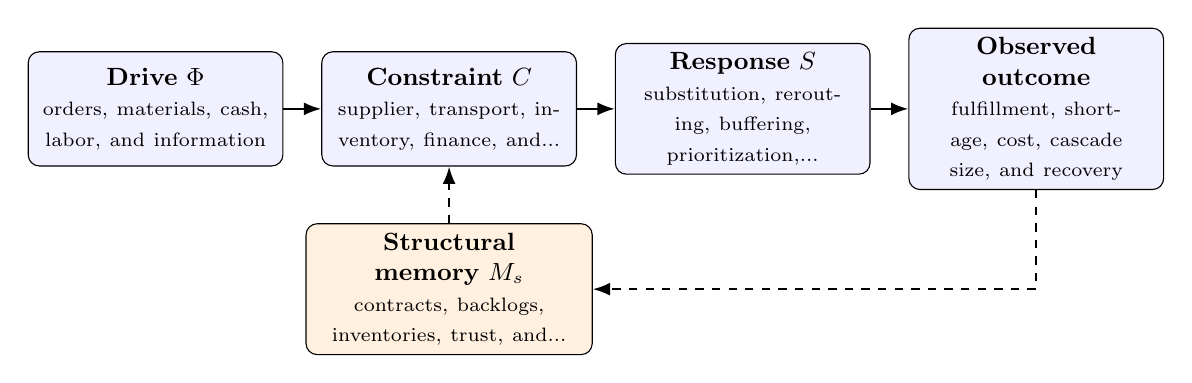
\begin{tikzpicture}[
    node distance=0.48cm,
    every node/.style={font=\small},
    box/.style={draw, rounded corners, align=center, minimum height=1.45cm, text width=3.0cm, fill=blue!6},
    memory/.style={draw, rounded corners, align=center, minimum height=1.25cm, text width=3.4cm, fill=orange!12},
    flow/.style={-{Latex[length=2.2mm]}, thick},
    feedback/.style={-{Latex[length=2.2mm]}, thick, dashed}
]
\node[box] (drive) {\textbf{Drive $\Phi$}\\\scriptsize orders, materials, cash, labor, and information};
\node[box, right=of drive] (constraint) {\textbf{Constraint $C$}\\\scriptsize supplier, transport, inventory, finance, and...};
\node[box, right=of constraint] (response) {\textbf{Response $S$}\\\scriptsize substitution, rerouting, buffering, prioritization,...};
\node[box, right=of response] (outcome) {\textbf{Observed outcome}\\\scriptsize fulfillment, shortage, cost, cascade size, and recovery};
\node[memory, below=0.72cm of constraint] (memory) {\textbf{Structural memory $M_s$}\\\scriptsize contracts, backlogs, inventories, trust, and...};
\draw[flow] (drive) -- (constraint);
\draw[flow] (constraint) -- (response);
\draw[flow] (response) -- (outcome);
\draw[feedback] (outcome.south) |- (memory.east);
\draw[feedback] (memory.north) -- (constraint.south);
\end{tikzpicture}
\caption{Paper D-11 observable CDFD/AFL architecture for Supply Chains. Solid arrows give the proposed forward chain; dashed arrows make history-dependent feedback explicit.}
\label{fig:d11-architecture}
\end{figure}

\subsection{Minimal Coupled Model}

A paper-level model must separate throughput, constraint accumulation, response,
and history. One deliberately minimal form is
\begin{align}
Y(t) &= \frac{\Phi(t)S(t)}{\epsilon + C(t)}, \\
\frac{dC}{dt} &= \alpha \Phi(t) - \beta S(t)C(t) + \gamma \mathcal{L}C(t), \\
\frac{dM_s}{dt} &= \eta C(t) - \mu M_s(t), \\
\Psi_s(t) &= \frac{\widehat{\Phi}(t)}{\epsilon+\widehat{C}(t)}\,
             \widehat{S}(t)\,[1+\omega\widehat{M_s}(t)] .
\end{align}
Here $Y$ is the measured output, $\epsilon>0$ prevents a singular denominator,
$\mathcal{L}$ is a spatial or network coupling operator, and hats denote
explicitly normalized variables. The sign and magnitude of $\omega$ must be
estimated: memory can preserve useful organization or amplify damage. No fixed
threshold is universal before the variables, normalization, and observation
scale are declared.

For this paper, the hypothesized causal sequence is specific. A change in
orders, materials, cash, labor, and information arrives faster than substitution, rerouting, buffering, prioritization, and coordination can compensate.
This raises or redistributes supplier, transport, inventory, finance, and production capacity. If the load persists,
the retained state encoded by contracts, backlogs, inventories, trust, and disruption history changes the next response, so a later event of equal
magnitude can produce a different trajectory in fulfillment, shortage, cost, cascade size, and recovery. The
scientific task is to estimate that sequence against the best ordinary model of
the domain, not merely to redescribe the outcome after it occurs.

\subsection{Cross-Scale Universality Without Mechanistic Erasure}

For the domain applications family, the universal comparison is a disciplined translation test across systems with very different material mechanisms. A valid mapping preserves the baseline science of the domain, declares the scale of every variable, and earns its place through a discriminating prediction rather than resemblance alone. \cite{Holling1973,Turing1952,Shannon1948,BakTangWiesenfeld1987}
The CDFD programme is cumulative: Part I supplies the flow--constraint
foundation \cite{MujjabiPartI2026}; Part II asks when maintained throughput
supports persistent organized states \cite{MujjabiPartII2026}; Part III
develops adaptive limitation and biological memory \cite{MujjabiPartIII2026};
and Part IV \cite{MujjabiPartIV2026} tests how much of that architecture
survives translation. The CDFD Runtime \cite{CDFDRuntime2026} supplies a
reproducible numerical stress surface, but it does not substitute for the
domain evidence named here.

The required scale declaration for this paper is hours to decades; facilities to global supply networks. At short
scales, the key question is whether the incoming drive is transmitted,
buffered, or diverted. At intermediate scales, response changes effective
capacity and network exposure. At long scales, retained structure can alter the
state space itself. A result is genuinely cross-scale only when the aggregation
rule is stated and the same conclusion is not an artifact of averaging.

\subsection{Evidence Ladder and Discriminating Tests}

\begin{table}[htbp]
\centering
\small
\caption{Evidence ladder for Paper D-11. Each rung can fail independently.}
\begin{tabularx}{\textwidth}{|p{0.17\textwidth}|X|X|}
\hline
\textbf{Test} & \textbf{Design} & \textbf{Discriminating result} \\
\hline
Proxy audit & Measure firm transactions, shipment traces, inventories, supplier networks, and disruption histories and preregister how each record maps to $\Phi$, $C$, $S$, $M_s$, and $Y$. & The mapping fails if proxies are non-identifiable, circular, or change meaning across cases. \\
\hline
Load ramp & Apply or observe a supplier or corridor failure under contrasting inventory histories while estimating the dominant constraint and response time. & A threshold claim requires a reproducible nonlinear change and uncertainty bounds, not a visually chosen breakpoint. \\
\hline
Recovery and memory & Match present load across units with different histories, then compare recovery paths. & The memory claim requires history-dependent divergence after current conditions are controlled. \\
\hline
Model comparison & Compare the baseline domain model with and without the CDFD/AFL state variables using held-out data. & The paper's stated falsifier is: memory and topology terms do not improve cascade or recovery prediction. \\
\hline
\end{tabularx}
\end{table}

The strongest practical design combines a prospective perturbation with a
recovery window. The load-ramp phase estimates where constraint begins to rise
faster than output. The recovery phase estimates $\beta$ and $\mu$, separating
fast relaxation from persistent memory. A topology or coupling intervention
then asks whether rerouting changes the cascade as predicted. Null results are
informative because they identify domains in which the universal notation adds
no measurable value.

\subsection{Research Programme and Boundary Conditions}

The immediate research programme has four steps. First, construct a documented
dataset from firm transactions, shipment traces, inventories, supplier networks, and disruption histories and retain raw units before normalization.
Second, fit a baseline domain model and report its calibration and out-of-sample
error. Third, add the smallest identifiable CDFD/AFL state extension and test
whether it improves prediction of fulfillment, shortage, cost, cascade size, and recovery. Fourth, repeat the
analysis across the declared scale range and publish negative cases as part of
the universality audit.

Three boundaries are non-negotiable. Correlation between flow and failure does
not identify a constraint mechanism. A fitted memory term does not prove that
the stored state has the same material meaning in another domain. Finally, a
runtime cascade is evidence about the implementation, not evidence that the
real system follows it. The paper becomes stronger when it can say precisely
where the translation stops.


% END PART IV MAJOR UNIVERSAL UPGRADE

\section{Conclusion}

Supply chains are multi-tier AFL networks. Goods throughput, inventory constraint, bullwhip
dynamics, JIT fragility, and cascade disruption all emerge from the universal AFL equation with
supply chain $(\Phi, C)$ interpretation. AFL connects supply chain management to all other
Part~IV papers through the universal flux--constraint framework, demonstrating that global supply
chains are the logistical substrate of civilisational AFL dynamics (Papers~25--34).

\bibliographystyle{plain}
\bibliography{universal_afl_references}

\end{document}